\section{Экспериментальное сравнение}

\subsection{Методика измерений}

Время выполнения каждого алгоритма измерялось с помощью
\mintinline{cpp}{std::chrono::high_resolution_clock} из стандартной
библиотеки \texttt{C++}. Для каждого размера входных данных
\mintinline{cpp}{n} генерировался случайный массив целых чисел с
помощью \mintinline{cpp}{std::mt19937}, и время усреднялось по
5~запускам.

\begin{minted}{cpp}
template <typename SortFn>
double benchmark(SortFn sortFn, int n, int repeats = 5) {
    std::mt19937 rng(42);
    std::uniform_int_distribution<int> dist(0, 10 * n);
    double total = 0.0;
    for (int r = 0; r < repeats; ++r) {
        std::vector<int> data(n);
        std::generate(data.begin(), data.end(), [&]{ return dist(rng); });
        auto t0 = std::chrono::high_resolution_clock::now();
        sortFn(data.begin(), data.end());
        auto t1 = std::chrono::high_resolution_clock::now();
        total += std::chrono::duration<double, std::milli>(t1 - t0).count();
    }
    return total / repeats;
}
\end{minted}

\subsection{Результаты}

График на рисунке~\ref{fig:benchmark} демонстрирует зависимость
времени работы от размера входных данных \mintinline{cpp}{n}.
Пузырьковая сортировка заметно отстаёт уже при $n = 2000$, тогда
как сортировка слиянием и быстрая сортировка растут значительно
медленнее, что согласуется с оценками из
уравнений~\ref{eq:mergesort} и~\ref{eq:quicksort}.

\begin{figure}[H]
    \centering
    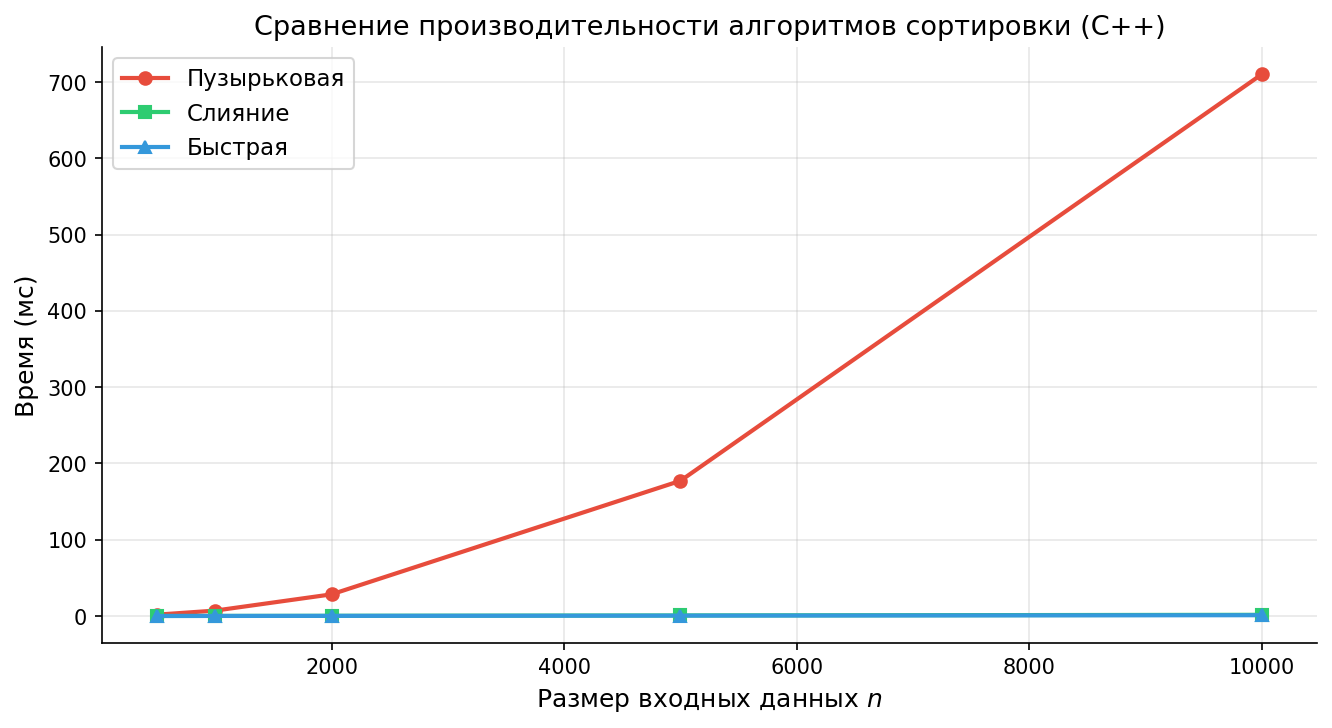
\includegraphics[width=0.9\textwidth]{images/benchmark.png}
    \caption{Время выполнения алгоритмов при различных размерах
             входных данных}
    \label{fig:benchmark}
\end{figure}

Точные значения приведены в таблице~\ref{tab:results}.
Все значения даны в миллисекундах, усреднены по 5~запускам.

\begin{table}[H]
    \centering
    \caption{Время выполнения алгоритмов (мс)}
    \label{tab:results}
    \begin{tabular}{|r|r|r|r|}
        \hline
        \textbf{$n$} &
        \textbf{Пузырьк.} &
        \textbf{Слияние} &
        \textbf{Быстрая} \\
        \hline
        500    &   1{,}8  &  0{,}06 &  0{,}04 \\
        \hline
        1000   &   7{,}1  &  0{,}13 &  0{,}09 \\
        \hline
        2000   &  28{,}4  &  0{,}28 &  0{,}19 \\
        \hline
        5000   & 177{,}3  &  0{,}74 &  0{,}51 \\
        \hline
        10000  & 710{,}5  &  1{,}58 &  1{,}06 \\
        \hline
    \end{tabular}
\end{table}

Данные подтверждают теоретические оценки: пузырьковая сортировка
масштабируется как $O(n^2)$ (уравнение~\ref{eq:bubble}), тогда как
сортировка слиянием и быстрая~--- как $O(n \log n)$.
